%\section{Resultados}

A Figura \ref{fig:acaoLPAEtDelta} mostra a aquisição feita de cinco(5) degraus de acionamento realizados sequencialmente, e como pode-se ver, há um sobressinal maior na resposta do primeiro degrau, sendo atenuado nos demais, pois houve um carregamento do registrador $\delta$ correspondente a correção da velocidade desejada.

%%%%%%%%%%%%%%%%%%%%%%%%%%%%%%%%%%%%%%%%%%%%%% Fig
\begin{figure}[!htb]%%%%%%%%%%%%%%%%%%%%%%%%%%%%%%
\caption{Ação de controle utilizando LPA$E\tau$}
\vspace{-1cm}\center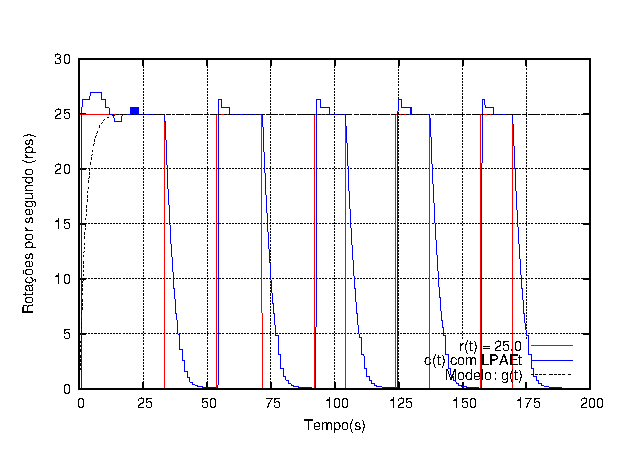
\includegraphics[scale=1.6]{./imagens/LPAEt-delta.eps}
\label{fig:acaoLPAEtDelta}

{\small Fonte: Próprio autor}
\end{figure}
%%%%%%%%%%%%%%%%%%%%%%%%%%%%%%%%%%%%%%%%%%%%%%%%%%


Ajustando os limiares, foi possível chegar ao resultado mostrado na Figura \ref{fig:LPAEterro}, 
onde pode-se comparar o resultado em dois momentos distintos, no primeiro e no segundo ciclo, comparativamente ao modelo gerado no Capítulo 3 deste trabalho.


%%%%%%%%%%%%%%%%%%%%%%%%%%%%%%%%%%%%%%%%%%%%%% Fig
\begin{figure}[!htb]%%%%%%%%%%%%%%%%%%%%%%%%%%%%%%
\caption{Erro na Ação de controle utilizando LPA$E\tau$}
\vspace{-1cm}\center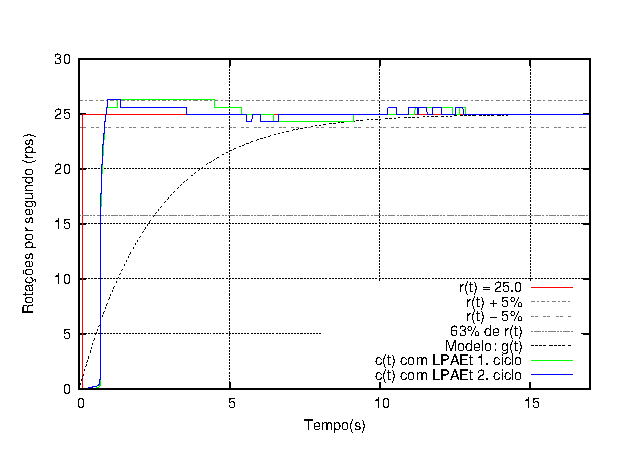
\includegraphics[scale=1.6]{./imagens/LPAEt-erro.eps}
\label{fig:LPAEterro}

{\small Fonte: Próprio autor}
\end{figure}
%%%%%%%%%%%%%%%%%%%%%%%%%%%%%%%%%%%%%%%%%%%%%%%%%%






A Figura \ref{fig:LPAEterro} mostra alguns parâmetros de 
referência, como o valor de referência, 
$r(t) = 25.0$ e linhas tracejadas indicando a 
tolerância adotada como critério de desempenho de 
$\pm $5\% além da curva do modelo do sistema.

O resultado obtido com o Controlador utilizando a 
LPA$E\tau$ proposta, é apresentada em duas partes,
um para cada ciclo de operação, 
pois, no primeiro ciclo, a variável de correção $\delta$
ainda não foi carregada, 
e o sistema apresenta um tempo de correção da contradição, 
já do segundo ciclo em diante, 
a resposta é mais rápida e mais acertiva pois já há um
valor de correção adequado, 
levando em consideração o ciclo anterior. 
Mesmo que não seja o mais adequado, 
deve ser o mais próximo do valor desejado, 
permitindo uma correção mais rápida, 
como se vê na resposta dos dois ciclos.


Para evidenciar o ganho de performance, 
foi calculado o erro relativo percentual médio,
da mesma forma como foi realizado para obtenção do modelo
do sistema em estudo, 
apresentado no Capítulo 4 deste trabalho.

A Tabela \ref{tab:ErroLPAEt} mostra para cada ciclo de 
acionamento do sistema, 
dois valores relativos ao período completo da amostragem e
desconsiderando o tempo relativo ao tempo de subida do sinal,
em que para ambos os ciclos, ocorre em $t = 0,88 s$, 
momento em que o sistema alcança o valor desejado, 
de referência.


%%%%%%%%%%%%%%%%%%%%%%%%%%%%%%%%%%%%%%%%%%%%%% Tab
\begin{table}[h]%%%%%%%%%%%%%%%%%%%%%%%%%%%%%%%%%%
\centering
\caption{Erro Relativo Percentual do controlador LPA$E\tau$}
\label{tab:ErroLPAEt}

\begin{tabular}{c|c|c}
\hline
Ciclo de Atuação & Intervalo de amostras  &  erro médio relativo \\ \hline
\hline
1º & 0,00 a 17,00 s &  5,44 \% \\ \hline
1º & 0,88 a 17,00 s &  1,90 \% \\ \hline
2º & 0,00 a 17,00 s &  4,41 \% \\ \hline
2º & 0,88 a 17,00 s &  0,82 \% \\ \hline
\end{tabular}

{\vspace{0.2cm} \small Fonte: Próprio autor}
\end{table}
%%%%%%%%%%%%%%%%%%%%%%%%%%%%%%%%%%%%%%%%%%%%%%%%%%

Como pode ser visto, há um ganho percentual de 
aproximadamento 1\% entre a atuação do primeiro 
para o segundo ciclo de acionamento. 


%%%%%%%%%%%%%%%%%%%%%%%%%%%%%%%%%%%%%%%%%%%%%%%%%%
%%%%%%%%%%%%%%%%%%%%%%%%%%%%%%%%%%%%%%%%%%%%%%%%%%
